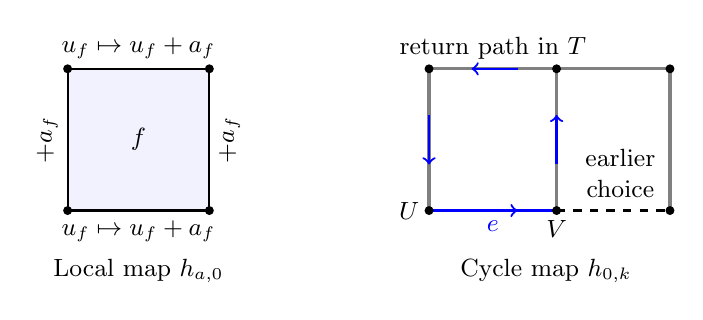
\begin{tikzpicture}[scale=.9, every node/.style={font=\small}]
  \begin{scope}
    \fill[blue!5] (0,0) rectangle (2,2);
    \draw[thick] (0,0)--(2,0)--(2,2)--(0,2)--cycle;
    \foreach \x/\y in {0/0,2/0,2/2,0/2}
      \fill (\x,\y) circle (1.8pt);
    \node at (1,1) {$f$};
    \node[below] at (1,0) {$u_f\mapsto u_f+a_f$};
    \node[above] at (1,2) {$u_f\mapsto u_f+a_f$};
    \node[rotate=90,above] at (0,1) {$+a_f$};
    \node[rotate=90,below] at (2,1) {$+a_f$};
    \node at (1,-.85) {Local map $h_{a,0}$};
  \end{scope}
  \begin{scope}[xshift=5.1cm]
    \coordinate (u) at (0,0);
    \coordinate (v) at (1.8,0);
    \coordinate (a) at (0,2);
    \coordinate (b) at (1.8,2);
    \coordinate (c) at (3.4,2);
    \coordinate (d) at (3.4,0);
    \draw[very thick,gray] (u)--(a)--(b)--(v);
    \draw[very thick,gray] (b)--(c)--(d);
    \draw[thick,blue] (u)--(v);
    \draw[thick,dashed] (v)--(d);
    \draw[->,blue,thick] (.6,0)--(1.25,0);
    \draw[->,blue,thick] (1.8,.65)--(1.8,1.35);
    \draw[->,blue,thick] (1.25,2)--(.6,2);
    \draw[->,blue,thick] (0,1.35)--(0,.65);
    \foreach \p in {u,v,a,b,c,d}
      \fill (\p) circle (1.8pt);
    \node[left] at (u) {$U$};
    \node[below] at (v) {$V$};
    \node[below,blue] at (.9,0) {$e$};
    \node[above] at (.9,2) {return path in $T$};
    \node[above,align=center] at (2.7,.05) {earlier\\choice};
    \node at (1.65,-.85) {Cycle map $h_{0,k}$};
  \end{scope}
\end{tikzpicture}
